\documentclass[10pt]{article}

\usepackage[T2A]{fontenc}
\usepackage[utf8x]{inputenc}

\usepackage[english,russian]{babel}
\usepackage{graphics, graphicx}

\usepackage[left=20mm, top=20mm, right=20mm, bottom=20mm, nohead, nofoot, footskip=15pt]{geometry}

\title{Отчёт по практикуму №1 }
\author{Дмитриев Леонид}


\begin{document}
	\maketitle
	
	\begin{abstract}
		\begin{center}
			Данный отчёт написан по практикуму, в котором исследовался алгоритм k ближайших
		    cоседей на датасете MNIST и подбирались параметры аугментации для улучшения предсказания.
		\end{center}
	\end{abstract}
	
	\begin{center} \section*{Список экспериментов} \end{center}
		
	\begin{itemize}
		\item {\bf Эксперимент 1}
			\subsubsection*{Дизайн эксперимента}
			{
				Целью является определение самого быстрого алгоритма для дальнейшего использования в экспериментах.\\
				Необходимо исследовать какой из алгоритмов поиска ближайших соседей работает быстрее при различных ситуациях.\\
				В эксперименте будет вестись поиск 5 ближайших соседей для каждого объекта тестовой выборки, а метрикой расстояния между объектами будет рассмотрена евклидова метрика. Будут исследованы следующие стратегии поиска: ручная реализация и библиотечные реализации: kd-tree, ball-tree, brute.\\
				Датасет будет формироваться из случайного подмножества признаков в количестве: 10, 20, 100.
	        }
	        
            \subsubsection*{Результаты эксперимента}
            {
                \begin{figure}[h]
            	    \begin{minipage}[h]{0.51\linewidth}
            		    \center{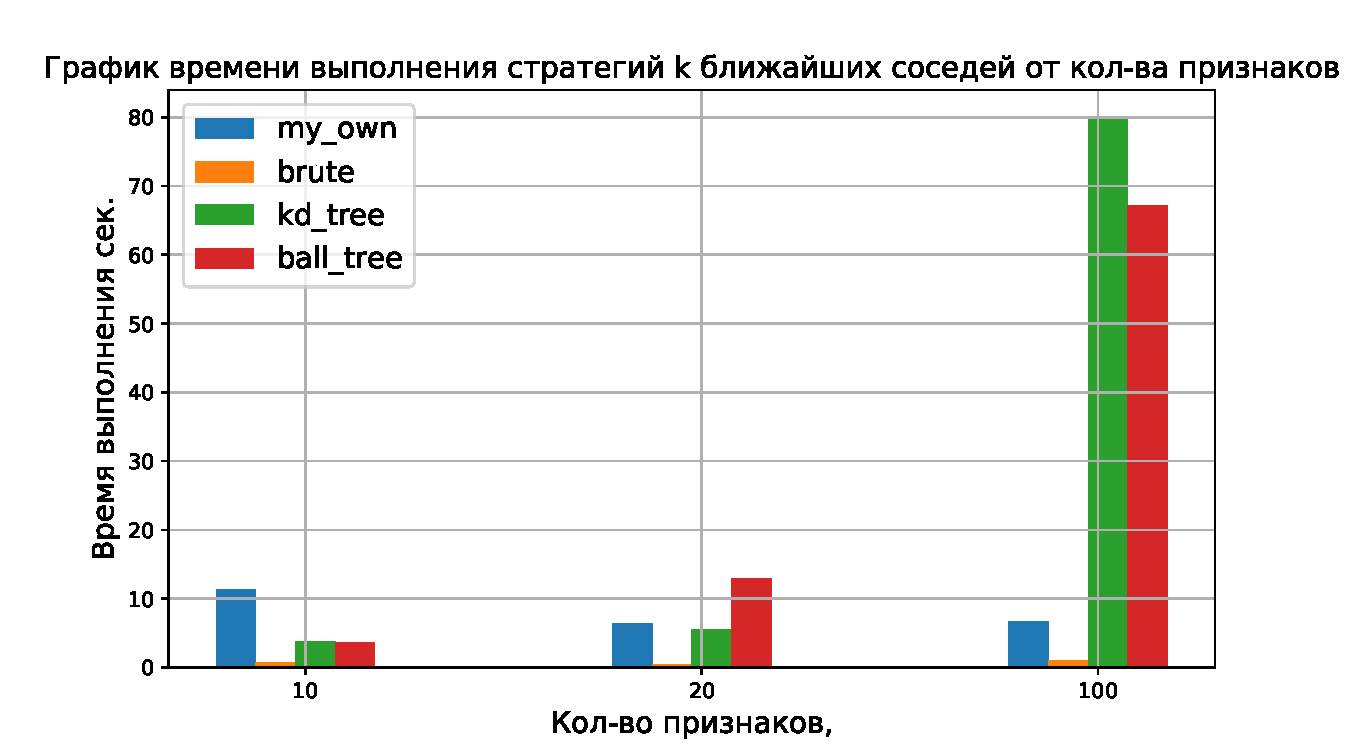
\includegraphics[width=1.0\linewidth]{experiment1_chart1.pdf}}
            	    \end{minipage}
            	    \hfill
            	    \begin{minipage}[h]{0.51\linewidth}
            		    \center{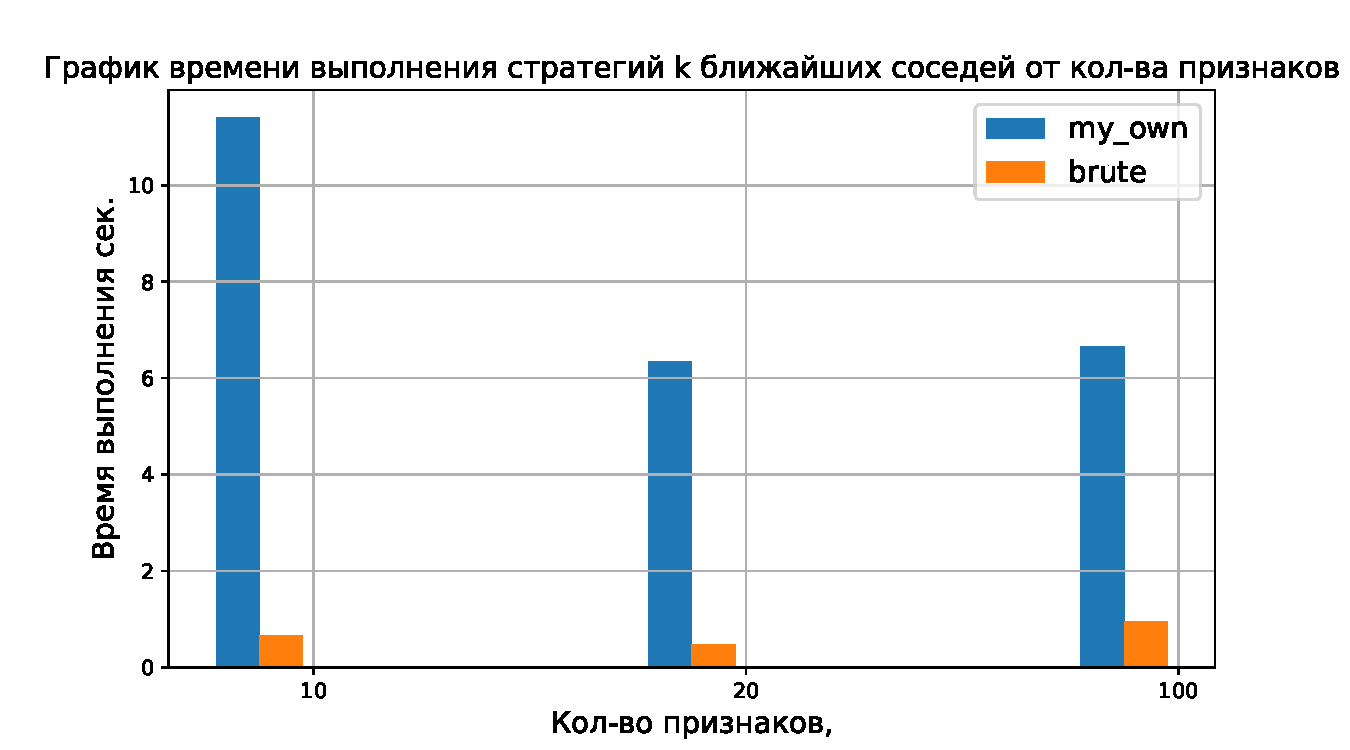
\includegraphics[width=1.0\linewidth]{experiment1_chart2.pdf}}
            	    \end{minipage}
            	    \caption{Exp. 1, Графики зависимости времени выполнения от числа признаков для разных алгоритмов}
            	    \label{ris:image1}
                \end{figure}
            }
	        
            \subsubsection*{Выводы из эксперимента}
            {
            	Был произведен подсчет времени нахождения 5 ближайших соседей для каждого объекта тестовой выборки с помощью алгоритмов: my-own, brute, kd-tree, ball-tree.\\
            	Алгоритм brute показал лучшее время, что объясняется простыми формулами  подсчета расстояний и быстрыми векторными операциями (для деревьев подобный подход не реализуем).\\
            	Собственная реализация примерно в 6-10 раз медленнее brute алгоритма на малых размерах (это можно объяснить большими временными затратами на создание процессов для параллелизации, когда в библиотечном brute это реализована более тонко), но асимптотика та же из-за одного и того же алгоритма (при росте размеров выборки их скорость близка друг к другу).\\
            	Алгоритмы на основе деревьев в данном эксперименте медленее brute в 60-80 раз.\\
            	На 10 и 20 признаках ball-tree медленее kd-tree в 2-5 раз, но при 100 признаках ball-tree работает в 1.17 раз быстрее kd-tree.
            }
			
		\item {\bf Эксперимент 2}
		    \subsubsection*{Дизайн эксперимента}
		    {
		    	Необходимо оценить по кросс-валидации на 3 фолдах точность и время работы алгоритма k ближайших соседей в зависимости от значений k с 1 до 10 и от евклидовой или косинусной метрики.\\
		    	Требуется выяснить какая из метрик даст лучший результат на рассматриваемом датасете и исследовать график точности от количества соседей на предмет выбросов (резких падений и улучшений точности).
		    }
		    
		    \subsubsection*{Результаты эксперимента}
		    {
		    	\begin{figure}[h]
		    		\begin{minipage}[h]{0.51\linewidth}
		    			\center{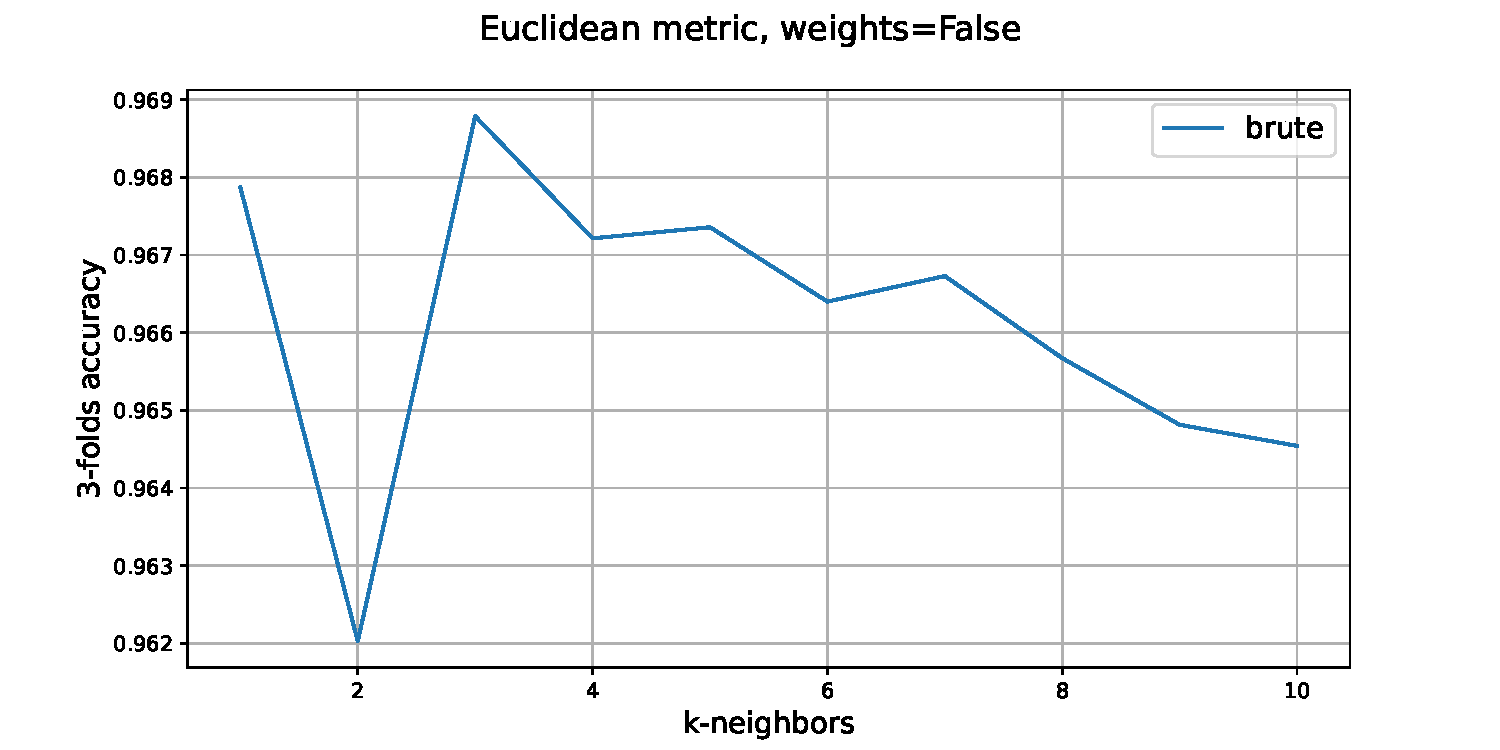
\includegraphics[width=1.0\linewidth]{experiment2_chart1.pdf}}
		    		\end{minipage}
		    		\hfill
		    		\begin{minipage}[h]{0.51\linewidth}
		    			\center{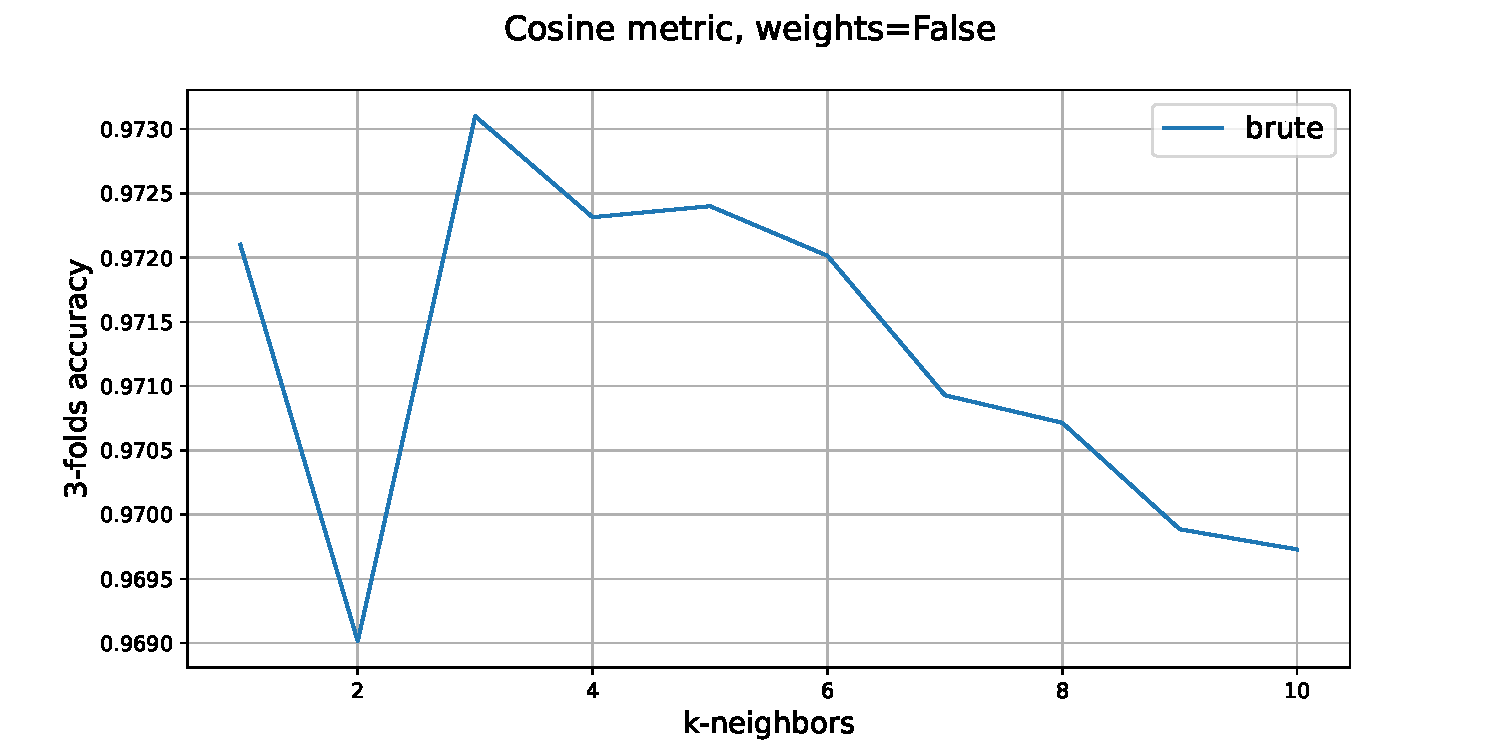
\includegraphics[width=1.0\linewidth]{experiment2_chart2.pdf}}
		    		\end{minipage}
	    		    \vfill
	    		    \begin{minipage}[h]{0.51\linewidth}
	    			    \begin{center}
	    			    	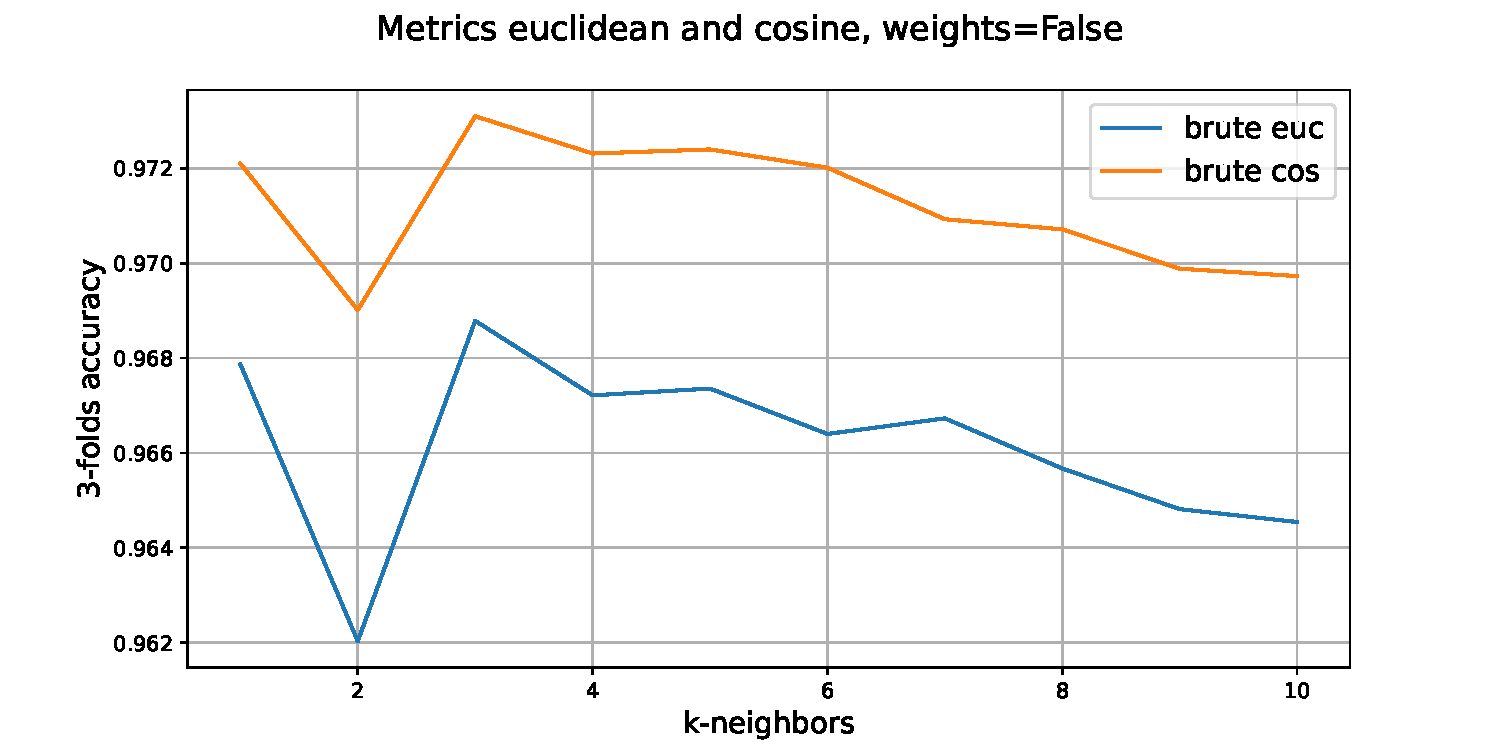
\includegraphics[width=1.0\linewidth]{experiment2_chart3.pdf}
	    			    \end{center}
	    		    \end{minipage}
		    		\caption{Exp. 2, Графики зависимости точности на 3 фолдах от количества соседей}
		    		\label{ris:image2}
		    	\end{figure}
		    }
		    
		    \subsubsection*{Выводы из эксперимента}
		    {
		    	Была произведена оценка точности алгоритма ближайших соседей по кросс-валидации с 3 фолдами при различных параметрах: k от 1 до 10, евклидова и косинусная метрики.\\
		    	Лучше всего себя показала косинусная метрика, которая превзошла евклидову при любом k от 1 до 10.\\
		    	Это могло произойти из-за того, что признаки в пустых пространствах равны нулю, а значит в скалярном произведении косинусной метрики учитываются различия только в тех координатах, которые несут информацию для обоих объектов, когда в евклидовой учитываются любые несовпадения.\\
		    	Это позволяет косинусной метрике учитывать только основной каркас символов и не отвлекаться на неровности по краям, отличающиеся на всех рисунках.\\
		    	На графиках зависимости точности от количества соседей для обеих метрик наблюдается резкий спад точности при количестве соседей равном 2. Это объясняется случайным выбором правильного ответа при равном количестве голосов каждого класса.
		    }
			
		\item {\bf Эксперимент 3}
		    \subsubsection*{Дизайн эксперимента}
		    {
		    	Необходимо произвести второй эксперимент, но на взвешенном алгоритме k ближайших соседей, и сравнить с обычным алгоритмом.
		    }
		    
		    \subsubsection*{Результаты эксперимента}
		    {
		    	\begin{figure}[h]
		    		\begin{minipage}[h]{0.51\linewidth}
		    			\center{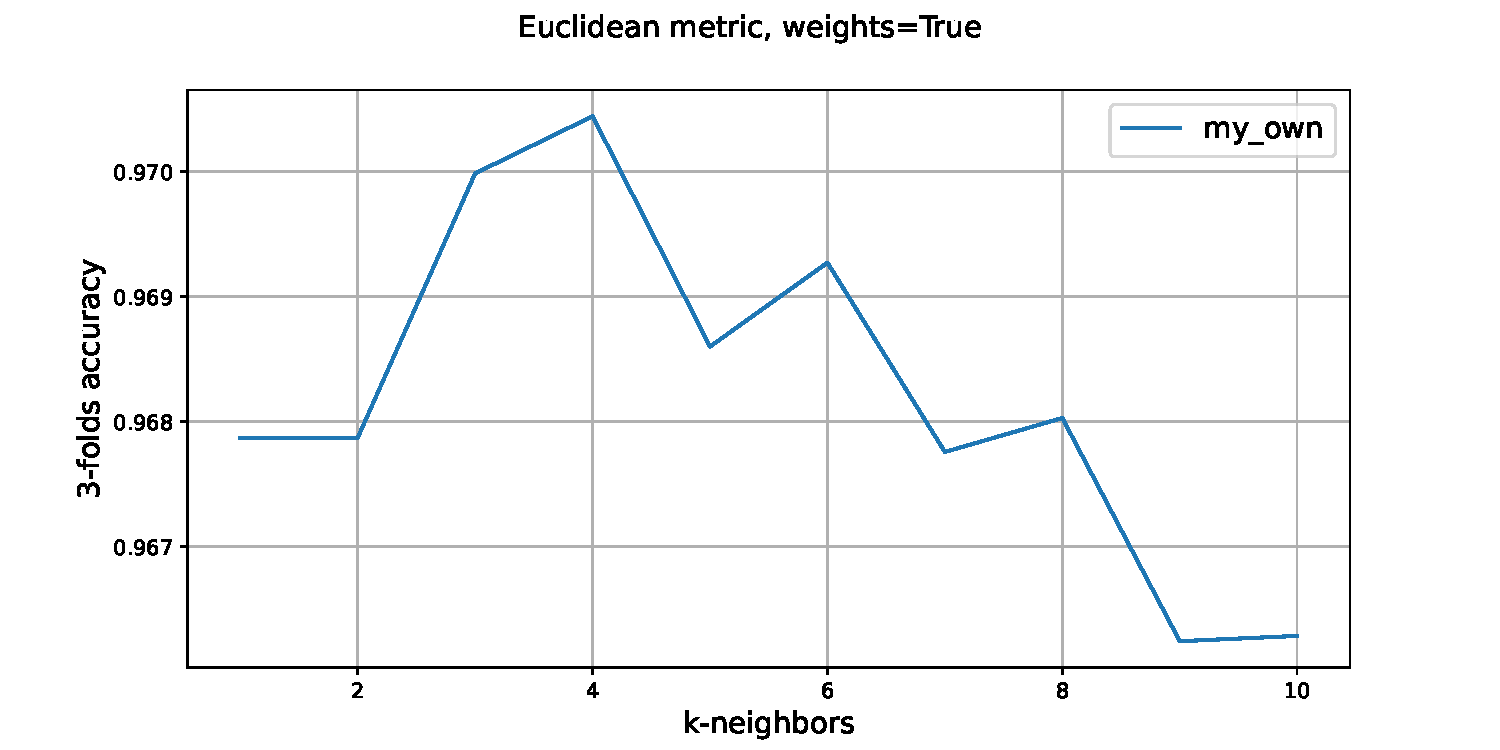
\includegraphics[width=1.0\linewidth]{experiment3_chart1.pdf}}
		    		\end{minipage}
		    		\hfill
		    		\begin{minipage}[h]{0.51\linewidth}
		    			\center{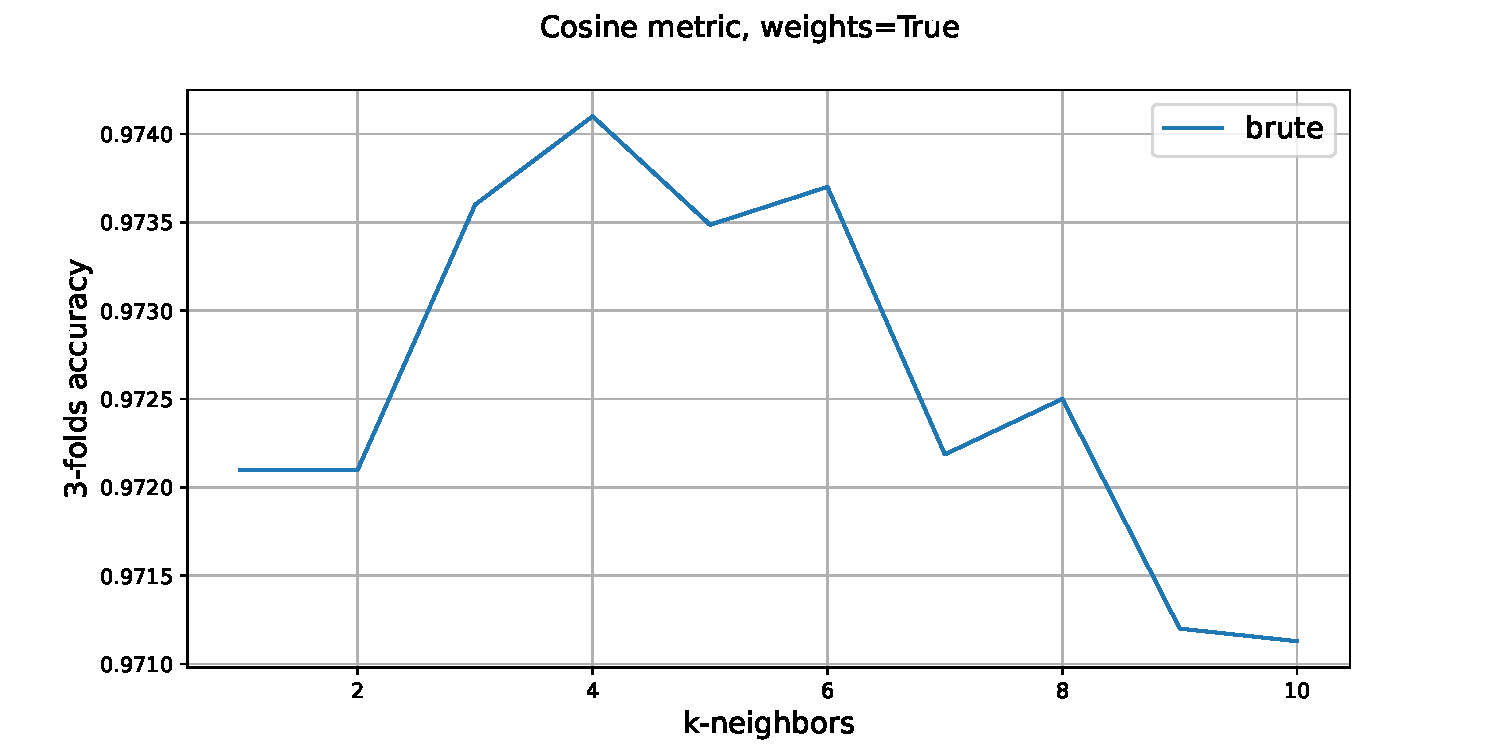
\includegraphics[width=1.0\linewidth]{experiment3_chart2.pdf}}
		    		\end{minipage}
		    		\vfill
		    		\begin{minipage}[h]{0.51\linewidth}
		    			\begin{center}
		    				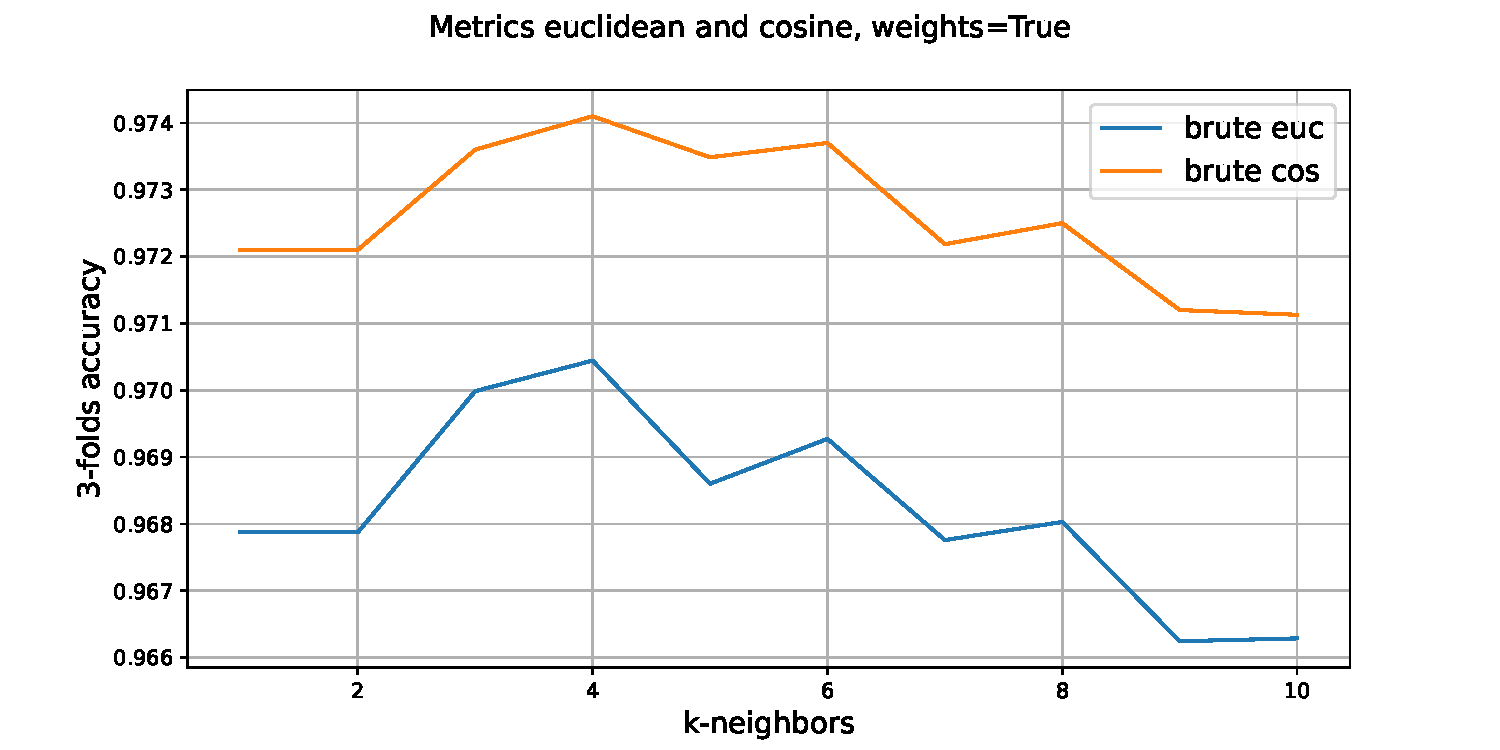
\includegraphics[width=1.0\linewidth]{experiment3_chart3.pdf}
		    			\end{center}
		    		\end{minipage}
		    		\caption{Exp. 3, Графики зависимости точности на 3 фолдах от количества соседей для взвешенного алгоритма}
		    		\label{ris:image3}
		    	\end{figure}
		    }
		    
		    \subsubsection*{Выводы из эксперимента}
		    {
		    	Была произведена оценка точности по кросс-валидации на 3 фолдах для взвешенного алгоритма k ближайших соседей на тех же параметрах, что и в 3 эксперименте.\\
		    	Взвешенный алгоритм показал себя лучше обычного на всех вариациях параметров (и совпал при 1 соседе). Лучшим алгоритмом оказался взвешенный my-own с 4  
		    	соседями на косинусной метрике.
		    }
			
		\item {\bf Эксперимент 4}
		    \subsubsection*{Дизайн эксперимента}
		    {
		    	Требуется исследовать лучший по результатам первых трех экспериментов алгоритм. Необходимо подсчитать точность и сравнить её с точностью по кросс-валидации, а также с точностью, указанной в интернете.\\
		    	Следует произвести анализ ошибок алгоритма, построив матрицу ошибок.\\
		    	Требуется визуализировать объекты, на которых допущены ошибки и выявить их общие черты.
		    }
		    
		    \subsubsection*{Результаты эксперимента}
		    {	    
		    	Лучший алгоритм: взвешенная собственная реализация на косинусной метрике с 4 соседями.\\
		    	Точность на дефолтном разбиении на тренировочную и тестовую выборки: 0.9752\\
		    	\begin{figure}[h]
		    		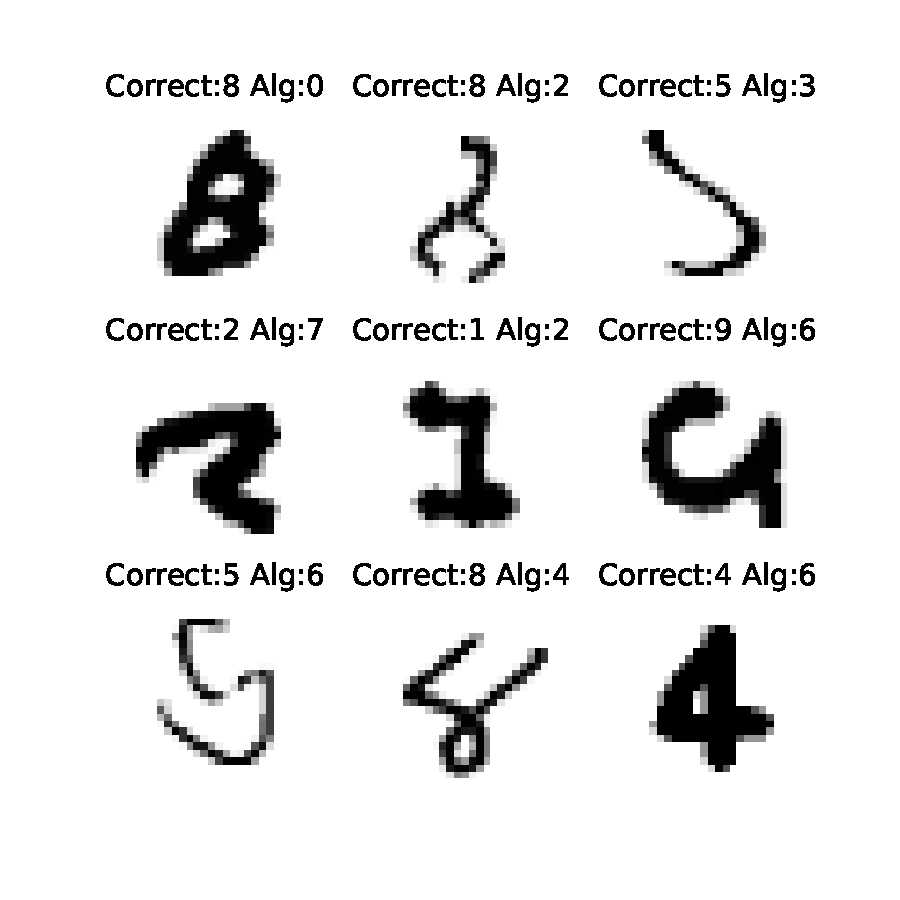
\includegraphics[width=9cm, height=9cm]{experiment4_errors_subset.pdf}
		    		\caption{Exp. 4, Некоторые объекты, на которых были допущены ошибки}
		    		\label{ris:image5}
		    	\end{figure}
		    }
		    
		    \subsubsection*{Выводы из эксперимента}
		    {
		    	На кросс-валидации в среднем алгоритм работает лучше, чем на изначальном разбиении, на 0.0007 секунд.\\
		    	По матрице ошибок можно понять, что алгоритм часто вместо 4 и 7 ставит 9. 3 принимает за 5. 7 принимает за 1.\\
		    	Из визуализации объектов, на которых были допущены ошибки, можно увидеть, что из объединяют некоторые особенности и дефекты: пропуски, большая толщина, неровный почерк, крутой наклон, поворот вокруг центра, отличающийся от среднего масштаб.
		    }
			
		\item {\bf Эксперимент 5}
		    \subsubsection*{Дизайн эксперимента}
		    {
		    	Требуется произвести аугментацию обучающей выборки. Необходимо использовать повороты, смещения, морфологические операции (эрозия, дилатация, открытие, закрытие с ядром 2), гауссовский фильтр.\\
		    	\\
		    	Величины преобразований, которые необходимо рассмотреть:\\
		    	1. Величина поворота: 5, 10, 15 градусов (в обе стороны)\\
		    	2. Величины смещения: 1, 2, 3 пикселя (по 4 направлениям осей)\\
		    	3. Дисперсия фильтра Гаусса: 0.5, 1, 1.5\\
		    	\\
		    	Необходимо по кросс-валидации на 3 фолдах подобрать параметры преобразований.\\
		    	Требуется проанализировать, какие ошибки алгоритма помогают исправить подобранные преобразования.
		    }
		    
		    \subsubsection*{Результаты эксперимента}
		    {
		    	При жадном поиске лучших преобразований была отобрана следующий набор комбинаций преобразования:
		    	\begin{itemize}
		    		\item
		    		\begin{itemize}
		    			\item
		    			Поворот на 5 градусов влево
		    			\item
		    			Дисперсия фильтра Гаусса с ядром из единиц 3 на 3 и параметром 1.0.
		    		\end{itemize}
		    		\item
		    		\begin{itemize}
		    			\item
		    			Поворот на 5 градусов вправо
		    			\item
		    			Дисперсия фильтра Гаусса с ядром из единиц 3 на 3 и параметром 1.0.
		    		\end{itemize}
	    		    \item
	    		    \begin{itemize}
	    		    	\item
	    		    	Поворот на 10 градусов вправо
	    		    	\item
	    		    	Дисперсия фильтра Гаусса с ядром из единиц 3 на 3 и параметром 1.0.
	    		    \end{itemize}
    		        \item
    		        \begin{itemize}
    		        	\item
    		        	Открытие с ядром 2
    		        	\item
    		        	Дисперсия фильтра Гаусса с ядром из единиц 3 на 3 и параметром 1.0.
    		        \end{itemize}
    	            \item
    	            \begin{itemize}
    	            	\item
    	            	Закрытие с ядром 2
    	            	\item
    	            	Дисперсия фильтра Гаусса с ядром из единиц 3 на 3 и параметром 1.0.
    	            \end{itemize}
                    \item
                    \begin{itemize}
                    	\item
                    	Дисперсия фильтра Гаусса с ядром из единиц 3 на 3 и параметром 1.0.
                    \end{itemize}
		    	\end{itemize}
	    	    Вместе они увеличивают размер тренировочной выборки в 6 раз, а качество (точность) предсказания на 3 фолдах достигает 0.9839.
		    }
		    
		    \subsubsection*{Выводы из эксперимента}
		    {
		    	Был проведен поиск преобразований для аугментации выборки по кросс-валидации на 3 фолдах.\\
		    	В полученных преобразованиях выделяется гауссовский фильтр, применяющийся для каждого преобразования. Это можно объяснить тем, что даже для двух похожих цифр существует разница не только в смещении по оси, но и разная кривизна линий. Именно эту разницу смягчает фильтр Гаусса. А закрытие и открытие добавляют более четкие очертания в выборку.
		    }
			
		\item {\bf Эксперимент 6}
		    \subsubsection*{Дизайн эксперимента}
		    {
		    	Требуется повторить поиск лучших преобразований на том же множестве параметров, что и в 5 эксперименте, но для тестовой выборки, не изменяя валидационную выборку.\\
		    	Необходимо проанализировать как изменилась матрица ошибок.\\
		    	Требуется качественно сравнить подходы экспериментов 5 и 6.
		    }
		    
		    \subsubsection*{Результаты эксперимента}
		    {
		    	Был произведен жадный поиск параметров преобразования тестовой выборки:
		    	\begin{itemize}
		    		\item поворот на 5 градусов вправо
		    		\item поворот на 5 градусов влево
		    		\item смещение на 1 пиксель вниз
		    		\item смещение на 2 пикселя вниз
		    		\item смещение на 1 пиксель вверх
		    		\item смещение на 2 пикселя вверх
		    		\item гауссовский фильтр с единичным ядром 3 на 1
		    		\item гауссовский фильтр с единичным ядром 1 на 3
		    	\end{itemize}
	    	    Аугментация тестовой выборки данными преобразованиями и последующее голосование по предсказаниям для каждой из них дает точность на дефолтном разбиении: 0.9724
	    	  
		    }
		    
		    \subsubsection*{Выводы из эксперимента}
		    {
		    	Был произведен поиск параметров для улучшения точности предсказания на дефолтном разбиении на тренировочную и тестовую выборки.\\
		    	В основном были подобраны преобразования смещения и поворота. Это
		    	показывает, что лучшую точность в этом эксперименте дают преобразования минимально изменяющие резкость изображения (из меняющих толщину и резкость использовался только фильтр Гаусса со слабыми параметрами).\\
		    	В сравнении с 5 экспериментом здесь точность стала меньше, чем при обычном предсказании. Это можно объяснить разницей в размерах между тренировочной и тестовой выборками (так как при преобразовании большой выборки, больше вероятность совпасть близким объектам).\\
		    	Сравнивая матрицы ошибок 4 и 6 экспериментов, можно заметить, что на 30 процентов уменьшилось кол-во ошибочного принятия 4 за 9, в два раза уменьшились ошибки принятия 3 за 5, на 60 процентов больше ошибок 7 и 9.
		    	
		    }

	\end{itemize}

    \begin{center} \section*{Общие выводы из работы} \end{center}
    В ходе работы было проведено исследование применения алгоритма k ближайших соседей к датасету изображений цифр "MNIST".\\
    Удалось достичь точности на кросс-валидации в 0.9839 с помощью подобранной аугментации выборки.
	
\end{document}

